\chapter{Kontrollieren}

\section{Testprotokoll}
Dieser Abschnitt protokolliert das Testkonzept (siehe Kapitel \ref{sec:testkonzept}).
\subsection{Manuelle Tests}
\label{sec:automated-tests}

\subsection{Automatisierte Tests}
\label{sec:manual-tests}
Die automatisierten Tests wurden mit MiniTest und Capybara geschrieben, wie von Redmine selbst
vorgegeben. Auch das laufen lassen der Tests basiert auf dem vom Redmine vorgegebenen Rake Task. Um die
Tests laufen zu lassen, muss man \bgmintinline{bash}{rake redmine:plugins:test NAME=gnosis} im Terminal
ausführen. Dabei wird der Name des Plugins angegeben, damit nur die Tests für dieses Plugin laufen. Im
\bgmintinline{bash}{bin} Verzeichnis befindet sich eine \bgmintinline{bash}{bin/test} Datei, welche
diesen Rake Task ausführt und den Output schön formatiert.
Der Output sieht dann ungefähr so aus:
\begin{center}
    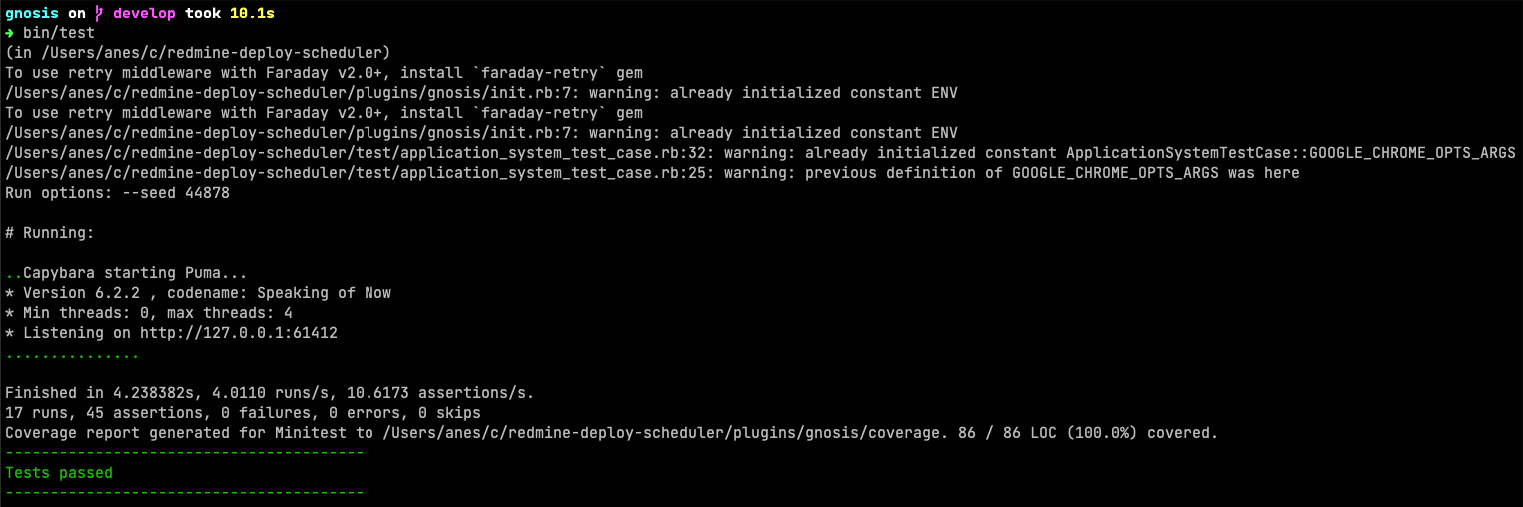
\includegraphics[width=0.75\textwidth]{images/misc/simplecov_terminal_output.png}
    \label{fig:simplecov_terminal_output}
\end{center}
SimpleCov generiert auch eine HTML Datei, in welcher die Coverage jeder Zeile genau markiert ist in
rot oder grün, je nachdem, ob es getestet wurde oder nicht. So sieht diese Datei in diesem Fall aus:
\begin{center}
    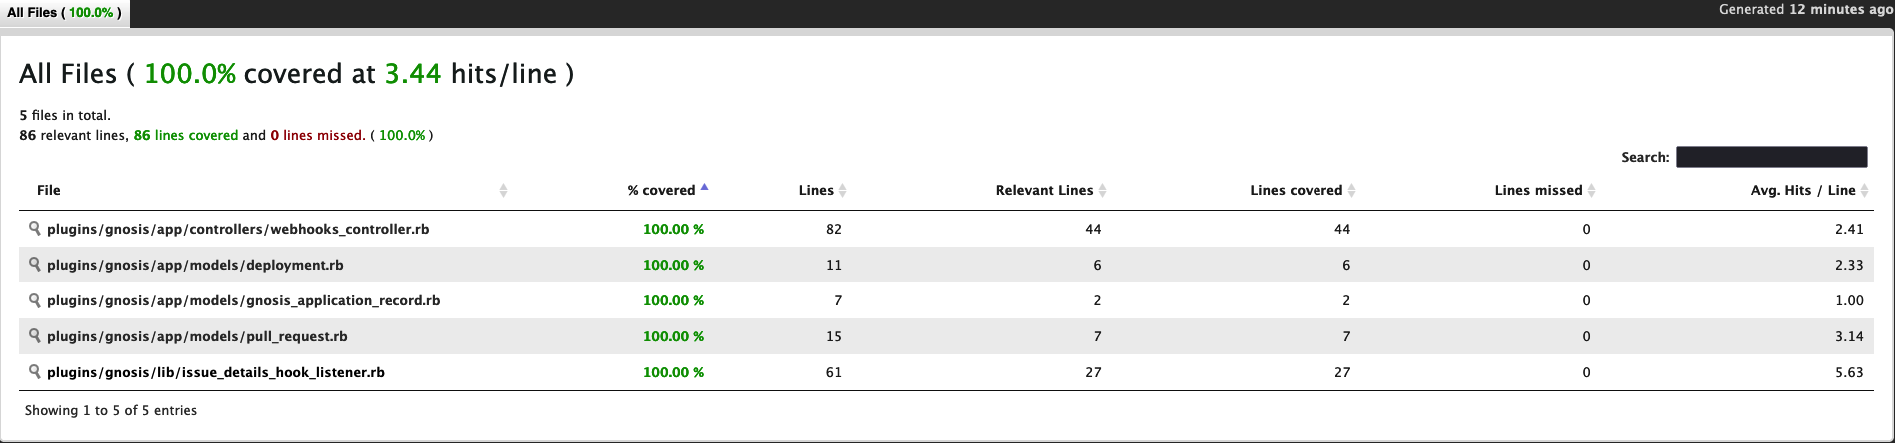
\includegraphics[width=0.75\textwidth]{images/misc/simplecov_html.png}
    \label{fig:simplecov_html_output}
\end{center}

\subsubsection{Verscheidene Testarten}
Die Tests befinden sich im \bgmintinline{bash}{test} Verzeichnis. Dort werden diese in verschiedene
Gruppen aufgeteilt, basierend auf der Testart. Die Gruppen sind:
\begin{itemize}
    \item \bgmintinline{bash}{functional} - Funktionale Tests senden Anfragen an die Controller.
    \item \bgmintinline{bash}{unit} - Unittests, welche die einzelnen Klassen und dessen Methoden
    testen.
    \item \bgmintinline{bash}{system} - System Tests klicken sich mit Capybara durch die UI des
    Plugins und testen so die Funktionalität.
\end{itemize}
Die funktionalen Tests wurden für das Testen des \bgmintinline{ruby}{class WebhooksController}
genutzt. Sie schicken Anfragen an den Controller und desssen Funktionen und testen so, ob die richtigen
Objekte basierend auf dem erstellt werden. \newline
Die Unittests wurden für das Testen der \bgmintinline{ruby}{class Deployment} und 
\bgmintinline{ruby}{class PullRequest} genutzt. Sie testen die einzelnen Methoden dieser Klassen und
prüfen, ob die Objekte richtig manipuliert werden. \newline
Die Systemtests werden für das Testen der UI genutzt. Mithilfe von Capybara wird ein Headless Browser
gestartet, welcher sich durch die UI klickt und so die Funktionalität testet.  

\section{Versionierung}
\subsection{Dokumentation}
\subsection{Programm}
\subsubsection{Selbstkritische PR Reviews}

\section{Kopplung vom Hauptprogramm}

